\documentclass[11pt]{article}

\usepackage[T1]{fontenc}
\usepackage[utf8]{inputenc}
\usepackage{mathptmx}
\usepackage[scaled=0.92]{helvet}
\usepackage{courier}
\usepackage[margin=1in]{geometry}
\usepackage{microtype}
\usepackage{booktabs}
\usepackage{listings}
\usepackage{xcolor}
\usepackage{tikz}
\usetikzlibrary{arrows.meta,positioning}
\usepackage{caption}
\usepackage{enumitem}
\usepackage{orcidlink}
\usepackage[numbers,sort&compress]{natbib}
\usepackage{hyperref}

\newcommand{\code}[1]{\texttt{\detokenize{#1}}}
\setlength{\emergencystretch}{3em}

\lstset{
  language=C,
  basicstyle=\ttfamily\small,
  keywordstyle=\color{blue!60!black},
  commentstyle=\color{green!40!black},
  columns=fullflexible,
  keepspaces=true,
  frame=single,
  framerule=0.3pt,
  xleftmargin=4pt,
  xrightmargin=4pt,
}


\title{From C\# Scripts to Packed C Zero-Indirection Physics: \\
A Cache-Optimized 2D Game Engine Architecture with Intrusive Execution}
\author{Brent S. Hartshorn \orcidlink{0009-0004-2853-655X}, and Gilead Cosman}


\begin{document}
\maketitle

\begin{abstract}
Unity's built-in 2D physics is an integration of the Box2D engine~\cite{unity_physics}. We build the
same kind of 2D game runtime from a different direction. Game scripts are written in a subset of
C\#, translated to a subset of C++ and then to C, and compiled together with a fork of Box2D v3 that
we call Box2D-Packed. Our goal is a 2D runtime that is faster than Unity's. This paper describes the
two techniques we use to get there and measures each of them. The first is data packing: public
handles shrink from 8 to 4 bytes, and the records the engine reads on every step are laid out by
measured access patterns. Measured with Cachegrind's exact cache simulation, last-level data cache
misses fall by up to 65\% on query-heavy scenes relative to Box2D v3, with unchanged instruction
counts and bit-identical simulation results. The second is an \emph{intrusive engine}: game logic
is compiled into the physics engine at documented points, so it runs while the engine's data is
still in cache, instead of through callbacks and event arrays. Injected pre-solve logic saves
1.3\% of instructions, and injecting a platformer's event handlers cuts L1 data misses by 2\%, with
identical game results. We also report where injection does not help: a per-body gravity hook that
reads game data costs 7.65\% more L1 misses, and event handlers followed by game work on the same
objects add last-level misses. We compare against Box2D v3, not yet against Unity, and describe the
measurements that remain.
\end{abstract}

\section{Introduction}

Game engines such as Unity let developers write gameplay in C\# and rely on built-in engines for
rendering and physics. For 2D games, Unity's physics is Box2D~\cite{unity_physics}, the open-source
engine by Erin Catto~\cite{catto_box2d}. Between the game code and Box2D, Unity adds a managed
runtime, component objects, and callbacks such as \code{OnCollisionEnter2D}.

Our project, crust~\cite{crust}, takes a different path to the same kind of game. Its
\code{unity_pack} tool reads a Unity-shaped project, meaning C\# scripts and \code{.unity} scene
files, and produces a small C program:

\begin{enumerate}[leftmargin=*,itemsep=2pt]
  \item The scripts, written in a subset of C\#, are translated to a subset of C++ by
        \code{cs2cpp}.
  \item The C++ subset is translated to C by \code{cpprust}, and checked by crust's C compiler.
  \item The C is compiled by gcc together with scene data tables and the physics engine.
\end{enumerate}

Nothing in the result is a general object runtime. Each script class becomes an array of small
packed structs, sized from the scene, and object references become array indices. Box2D-Packed is
the 2D physics engine of this pipeline. Our goal is a 2D game runtime that is faster than Unity's,
while accepting the same kind of C\# the game developer already writes. This paper covers the
physics side of that goal. We have not yet run a comparison against Unity itself, and we say so
where it matters.

Box2D-Packed makes two kinds of changes to Box2D v3:

\begin{itemize}[leftmargin=*,itemsep=2pt]
  \item \textbf{Data packing.} Smaller public handles and structures, and a layout of the engine's
        internal records that follows measured access patterns (Sections~\ref{sec:packing}
        to~\ref{sec:negative}).
  \item \textbf{The intrusive engine.} A build pipeline that compiles game code into the engine at
        marked points, so game logic runs where the engine produces events
        (Section~\ref{sec:intrusive}), and its use as the physics backend of \code{unity_pack}
        (Section~\ref{sec:unity}).
\end{itemize}

We measure everything with deterministic cache simulation and require simulation results to stay
bit-identical to Box2D v3, unless a change is meant to alter behavior. We report negative results
in the same detail as positive ones, because several of them changed our design.

\section{Background and Concepts}
\label{sec:background}

This section introduces the ideas the rest of the paper relies on, for readers who have not worked
on game engines or low-level performance.

\subsection{What a physics step does}

A 2D physics engine advances the simulation in fixed time steps, typically 60 per second. Each
step has roughly four phases:

\begin{enumerate}[leftmargin=*,itemsep=2pt]
  \item \textbf{Broad phase.} Find pairs of shapes whose bounding boxes overlap. Box2D keeps the
        boxes in a tree (a bounding volume hierarchy) so it does not test every pair.
  \item \textbf{Narrow phase.} For each overlapping pair, compute the exact contact: whether the
        shapes touch, where, and along which normal. The result is a \emph{contact manifold}.
  \item \textbf{Solver.} Compute the forces that keep touching bodies from passing through each
        other, and integrate velocities and positions.
  \item \textbf{Events.} Report what happened to the game: which pairs started or stopped touching,
        which shapes entered sensors, which impacts were hard.
\end{enumerate}

Games attach their own logic to these phases: a \emph{custom filter} decides whether two shapes may
collide at all, and a \emph{pre-solve} callback may disable a contact just before it is solved,
which is how one-way platforms work.

\subsection{Handles instead of pointers}

Game code needs to refer to bodies and shapes that live inside the engine. Box2D v3 does not give
out pointers. It gives out \emph{handles}: an index into the engine's internal array, plus a
\emph{generation} number that is incremented whenever a slot is reused. If the game keeps a handle
to a destroyed body, the generation no longer matches, and the engine can detect the stale handle
instead of corrupting memory. The size of a handle matters because games store many of them.

\subsection{Caches, cache lines, and misses}

A CPU does not read single bytes from main memory. It reads 64-byte blocks called \emph{cache
lines} into a hierarchy of caches: a small, fast level-1 (L1) cache per core and a large, slower
last-level cache (LL). Reading data that is not in L1 is an \emph{L1 miss} and costs roughly tens of
cycles. Reading data that is not in any cache is a \emph{last-level miss} and costs one or two
hundred cycles, because it goes to main memory. Two consequences shape this paper:

\begin{itemize}[leftmargin=*,itemsep=2pt]
  \item Fields read together should sit in the same cache line. A record whose hot fields are
        spread over three lines costs three misses where one would do.
  \item A cache is divided into \emph{sets}, and each line can live only in the set its address
        maps to. If a loop visits records whose size is a power of two, the same field of every
        record can map to the same few sets, and those sets thrash while the rest of the cache sits
        idle. This is called set aliasing.
\end{itemize}

Hardware \emph{prefetchers} detect sequential access and load the next lines early, which hides
most of the cost of streaming through an array. Random access, such as looking up an object by
index, cannot be predicted and pays the full miss cost.

\subsection{Intrusive data structures}

The name of our build pipeline comes from a C++ idea. A \emph{non-intrusive} container, such as a
\code{std::list} of objects, keeps its bookkeeping outside the objects: each list node holds a
pointer or a copy, and the objects know nothing about the list. An \emph{intrusive} container
stores the bookkeeping inside the objects themselves~\cite{boost_intrusive}. An intrusive linked
list puts the \code{next} and \code{prev} links in each element, so walking the list reads only the
elements, not separate nodes. The same idea applies to reference counting: \code{std::shared_ptr}
keeps its count in a separate control block, while an \emph{intrusive pointer}
(\code{boost::intrusive_ptr}) keeps the count as a field of the object, so there is no extra
allocation and no extra memory read.

The trade is the same in both cases. An intrusive design gives up separation, because the object
now knows about its container, and gains locality and fewer indirections. We apply that trade to
the boundary between a game and its physics engine. Normally the game sits outside the engine and
learns about events afterwards, through callbacks or arrays. In an \emph{intrusive engine}, the
game's handlers are compiled into the engine's own loops, at the points where the engine already
holds the relevant data.

\subsection{Callbacks, event arrays, and link-time optimization}

A \emph{callback} is a function pointer the game registers with the engine. The engine calls it
for every relevant pair or contact. An indirect call through a pointer cannot be inlined by the
compiler, and the callback usually has to look up the game's own data by handle. An \emph{event
array} avoids the indirect call: the engine writes one entry per event during the step, and the
game reads the entries afterwards. By then the engine's data for that event has often left the
cache. \emph{Link-time optimization} (LTO) lets the compiler optimize across source files as one
program, which enables inlining between files that are compiled separately.

\section{Box2D v3}

Box2D v3 is already designed for cache efficiency. It keeps awake bodies in contiguous arrays of
body records (\code{b2BodySim}) and compact 32-byte body states used by the solver. Contacts that
touch are distributed over \emph{graph colors}, so that no two contacts in one color share a moving
body, and each color is solved in parallel with SIMD, 4 or 8 contacts at a time. The narrow phase
(\code{b2CollideTask}) visits every awake contact each step, updates its manifold or reuses it when
relative motion is small (contact recycling), and records which contacts started or stopped
touching. The engine then processes those changes on a single thread and creates begin and end
events.

\section{Methodology}
\label{sec:method}

\paragraph{Timing was not precise enough.} We first compared wall-clock times across the 14 scenes
of the Box2D benchmark suite. On one shared core, run-to-run noise ranged from 0.3--3.7\% in a quiet
session to 5--10\% in a busy one. Interleaving the builds and pairing runs did not reduce the noise
enough to resolve the 2--5\% effects that layout changes produce.

\paragraph{Cachegrind.} We therefore measure with Cachegrind~\cite{nethercote2007valgrind}, which
simulates the cache hierarchy for every memory access. We fix the simulated hierarchy at a 32\,KB
8-way L1 data cache, an 8\,MB 16-way last-level cache, and 64-byte lines, so results do not depend
on the host. A repeated run reproduced every counter to the last digit, so any difference between
builds is real. We report instructions, L1 data misses, and last-level data misses.

\paragraph{Limits of the method.} Cachegrind does not model hardware prefetchers. It counts one
miss per line for a sequential stream that a real CPU would mostly hide, while it models random
access well. All measurements use one worker thread. The results show where memory traffic
changes, but they do not predict time on a particular CPU.

\paragraph{Correctness.} Every change passes Box2D's unit tests in release and debug builds,
including a cross-platform determinism test against a fixed state hash, worker-count parity
checks, and snapshot and replay round trips. Every injection demo builds the same game both ways,
through the standard API and through injection, and requires identical results.

\section{Data Packing}
\label{sec:packing}

\paragraph{Handles.} Body, shape, chain, and joint handles store a 16-bit index and a 16-bit
generation, 4 bytes in total, where Box2D v3 uses 8 (Table~\ref{tab:handles}). The world index is
removed, so Box2D-Packed supports one world at a time, enforced at compile time. Contact handles
keep 32-bit fields, 8 bytes instead of 12, because large piles exceed 65{,}535 contacts and
contacts churn fast enough that a 16-bit generation would wrap quickly. Creating more than 65{,}535
live objects of one kind logs an error and returns a null handle, instead of silently wrapping onto
an existing object.

\begin{table}[ht]
\centering
\caption{Handle sizes in bytes.}
\label{tab:handles}
\begin{tabular}{lrr}
\toprule
Handle & Box2D v3 & Box2D-Packed \\
\midrule
Body, shape, chain, joint & 8 & \textbf{4} \\
Contact & 12 & \textbf{8} \\
World & 4 & 4 \\
\bottomrule
\end{tabular}
\end{table}

\paragraph{Definitions and filters.} Boolean flags in the creation structures become 1-bit
\code{bool} fields. We use \code{bool} rather than \code{uint8_t} bit-fields because C converts any
non-zero value to 1 when storing into a \code{bool}, while a 1-bit unsigned field keeps only the
low bit and silently stores 0 for a value such as \code{0x2}. Fields are ordered by alignment.
Collision filters use 16-bit category and mask fields, as in Box2D v2, which reduces
\code{b2Filter} from 24 to 6 bytes (Table~\ref{tab:structs}). None of these structures is read
during the simulation step, so, as expected, a timing comparison after this phase showed no
difference beyond noise.

\begin{table}[ht]
\centering
\caption{Structure sizes in bytes, 32-bit float build.}
\label{tab:structs}
\begin{tabular}{lrr}
\toprule
Structure & Box2D v3 & Box2D-Packed \\
\midrule
\code{b2Filter} & 24 & \textbf{6} \\
\code{b2QueryFilter} & 16 & \textbf{4} \\
\code{b2ShapeDef} & 88 & \textbf{56} \\
\code{b2BodyDef} & 88 & \textbf{72} \\
\code{b2ChainDef} & 88 & \textbf{64} \\
\code{b2DistanceJointDef} & 128 & \textbf{112} \\
\code{b2RevoluteJointDef} & 120 & \textbf{104} \\
\midrule
\code{b2Shape} (internal) & 280 & \textbf{264} \\
\code{b2TreeProxy} (internal) & 24 & \textbf{16} \\
\code{b2ContactSim} (internal) & 200 & \textbf{192} \\
\bottomrule
\end{tabular}
\end{table}

\section{Hot-Path Layout}
\label{sec:hotpath}

We used per-function and per-line Cachegrind annotations to find where misses occur, then changed
the layout of the records read there.

\paragraph{Category bits in tree nodes.} A tree query tested each overlapping leaf's category bits
through a separate proxy array, a second random access per leaf, even for leaves the filter
rejects. A 2D tree node has 8 unused bytes, which hold the z bounds in 3D. We store leaf category
bits there, so queries test the node they have already loaded, and only leaves that pass the filter
read the proxy. The \code{tree_cast} scene, which does not touch shapes, isolates this change: L1
data misses fall 2.9\%, last-level misses 7.3\%, and instructions 0.4\%.

\paragraph{A hot cache line in \code{b2Shape}.} The broad-phase pair filter read fields at offsets
4, 16, 20, 92, and 256 of each shape, three cache lines per shape. We moved every field the filter
reads into the first 64 bytes, so the filter now reads one line.

\paragraph{Power-of-two aliasing.} Packing the shape's flags into bits made \code{b2Shape} exactly
256 bytes, and Cachegrind showed last-level misses in \code{large_pyramid} rising 26.9\%. The
increase came from \code{b2ComputeFatShapeAABB}, which does not read any moved field. With a
256-byte stride, one field of every shape falls into only a quarter of the cache sets, and the loop
that sweeps all shapes each step thrashes those sets. Keeping plain \code{bool} flags gives 264
bytes, shifts each shape by 8 bytes, and spreads the fields over all sets. At 264 bytes, the
regression disappeared (+0.1\%), and the gains elsewhere roughly doubled: relative to the previous
step, \code{tile_world} last-level misses fell 62.5\% rather than 36\%, and \code{queries} 57\%
rather than 25\%. A compile-time assertion now keeps the size from returning to a power of two.

\paragraph{Narrow phase.} \code{b2CollideTask} read \code{bodyId} from both shapes of every contact,
two random cache lines, although the value is needed only in a rare fallback for sleeping bodies.
We now read the shape only in that branch, and moved the body fields the narrow phase reads to the
first 40 bytes of \code{b2BodySim}. L1 data misses fell by 1.0--3.4\% in scenes with contacts.

\paragraph{A three-line contact record.} At 200 bytes, most contact records straddled a fourth
cache line. The GJK simplex cache (8 bytes) is used only by chain-segment collisions, so we moved
it to the cold per-contact record, which made \code{b2ContactSim} exactly 192 bytes, three lines.

\paragraph{Cumulative result.} Table~\ref{tab:cumulative} compares Box2D-Packed with Box2D v3.
Last-level data misses fall in every scene, from 1.6\% in \code{many_pyramids} to 65.3\% in
\code{tile_world}, and instruction counts change by at most 0.4\%. The largest gains are in
query-heavy scenes. The table was measured before the injection markers of
Section~\ref{sec:intrusive} were added. The markers compile to nothing in normal builds, and results
stay bit-identical, but we have not re-run the table since.

% Generated by make_cachegrind_table.py, do not edit
\begin{table}[t]
\centering\small
\caption{Box2D-Packed relative to Box2D v3 under Cachegrind (32\,KB L1, 8\,MB LL, one worker).
Changes of 5\% or more are in bold. Negative is better.}
\label{tab:cumulative}
\begin{tabular}{lrrr}
\toprule
Scene & Instr. & L1 data & LL data \\
\midrule
\texttt{tile\_world} & $-$0.1\% & \textbf{$-$25.7\%} & \textbf{$-$65.3\%} \\
\texttt{queries} & +0.2\% & \textbf{$-$8.6\%} & \textbf{$-$56.7\%} \\
\texttt{tree\_cast} & $-$0.4\% & $-$2.8\% & \textbf{$-$7.3\%} \\
\texttt{smash} & +0.3\% & $-$2.7\% & \textbf{$-$5.4\%} \\
\texttt{large\_pyramid} & +0.2\% & $-$3.6\% & \textbf{$-$18.0\%} \\
\texttt{many\_pyramids} & +0.2\% & $-$3.6\% & $-$1.6\% \\
\texttt{joint\_grid} & +0.0\% & $-$0.3\% & $-$4.3\% \\
\bottomrule
\end{tabular}
\end{table}


\section{Negative Results}
\label{sec:negative}

\paragraph{Ordering contacts within a color.} The wide contact solver accounts for 64\% of L1 read
misses in \code{large_pyramid}. Because a body appears at most once per graph color, the order of
contacts within a color cannot change results. We sorted each color by body index, expecting the
solver's body reads to become sequential. All determinism tests passed, and the solver's misses
were identical to the last digit (95{,}726{,}000). The misses we had attributed to body reads were
the first touch of each 592-byte constraint bundle in a sequential sweep, which prefetchers largely
hide on real hardware. The sort cost 10.4\% more instructions and was dropped.

\paragraph{Removing inverse mass copies.} Removing four inverse-mass copies from
\code{b2ContactSim} also produced a 192-byte record with bit-identical results and cut
\code{large_pyramid} last-level misses 23.3\%. It raised L1 misses 3.3\% and instructions 0.6\%,
because contact preparation then read body records at random, and \code{many_pyramids} came out net
worse. Moving the simplex cache reached the same size without these costs.

\section{The Intrusive Engine}
\label{sec:intrusive}


\begin{figure}[ht]
\centering
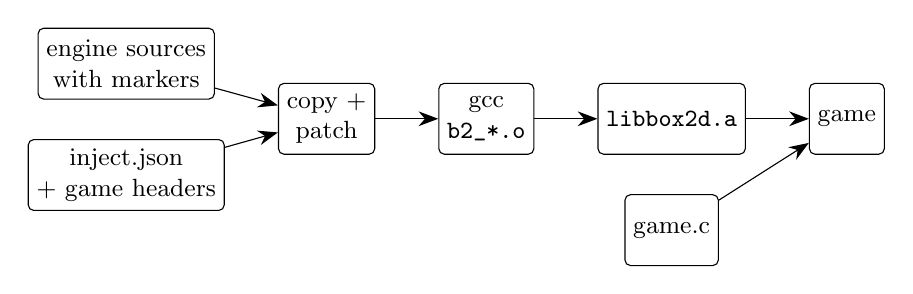
\begin{tikzpicture}[
  node distance=5mm and 8mm,
  box/.style={draw, rounded corners=2pt, align=center, font=\small, minimum height=9mm, inner sep=3pt},
  arr/.style={-{Stealth[length=2.5mm]}}
]
\node[box] (src) {engine sources\\with markers};
\node[box, below=of src] (json) {inject.json\\+ game headers};
\node[box, right=of src, yshift=-7mm] (patch) {copy +\\patch};
\node[box, right=of patch] (cc) {gcc\\\code{b2_*.o}};
\node[box, right=of cc] (lib) {\code{libbox2d.a}};
\node[box, right=of lib] (exe) {game};
\node[box, below=of lib] (user) {game.c};
\draw[arr] (src) -- (patch);
\draw[arr] (json) -- (patch);
\draw[arr] (patch) -- (cc);
\draw[arr] (cc) -- (lib);
\draw[arr] (lib) -- (exe);
\draw[arr] (user) -- (exe);
\end{tikzpicture}
\caption{The intrusive engine build pipeline.}
\label{fig:pipeline}
\end{figure}
\subsection{Pipeline}

The engine sources contain marker comments of the form \code{//$scope$POINT} on lines of their
own. A normal build ignores them. The script \code{box2d_pack.py} copies the sources, replaces
markers in the copies with C code described by a JSON file, and compiles the engine and the game
together (Figure~\ref{fig:pipeline}). Compiler errors point at the JSON entry, not the patched copy,
and the game's own headers can be included, so injected code can use the game's types and inline
functions directly.


A one-way platform, for example, is injected as follows. The game's rule is a \code{static inline}
function in its own header, and the pre-solve marker calls it with the two shapes the engine is
already holding:

\begin{lstlisting}[language={}]
{
  "includes": [ "platformer.h" ],
  "defines": { "B2_PACK_NO_PRE_SOLVE_FCN": 1 },
  "inject": [ {
    "event": "pre_solve",
    "code": [ "Game_PreSolve( shapeA->userData, shapeB->userData,",
              "               &contactSim->manifold );" ]
  } ]
}
\end{lstlisting}

\subsection{Injection points and their contract}

Table~\ref{tab:markers} lists the injection points. Each documents its thread context and the
variables injected code may use. Two run on worker threads and must be thread-safe, and the build
tool prints a note whenever code is injected there. Where the engine uses a concept in several
places, the marker lives in one inline hook that every place calls, so injected logic applies
consistently. The custom filter, for example, applies to new contacts, sensor overlaps, and
continuous collision.

\begin{table}[ht]
\centering
\caption{Injection points.}
\label{tab:markers}
\begin{tabular}{lll}
\toprule
Event & Runs & Typical use \\
\midrule
\code{pre_step}, \code{post_step} & main thread, world unlocked & game update \\
\code{contact_begin}, \code{contact_end} & single thread, world locked & damage, scoring \\
\code{contact_hit} & single thread, world locked & impact effects \\
\code{sensor_begin}, \code{sensor_end} & single thread, world locked & pickups, triggers \\
\code{custom_filter} & worker threads & teams, pass-through \\
\code{pre_solve} & worker threads & one-way platforms \\
\code{body_gravity} & worker threads, every substep & gravity fields \\
\bottomrule
\end{tabular}
\end{table}

Each marker is verified by an equivalence test that builds one scene with the standard callbacks
and event arrays, and again with injection, and requires identical output, including every body's
final position. A control build without the filter and pre-solve rules must produce a different
result, which shows the test is sensitive to those rules. The equivalence test found a bug in our
first gravity hook: it changed only velocity integration, while continuous collision also uses a
body's gravity scale when it rolls a fast body back to its time of impact. The \code{unity_pack}
integration found a second marker bug, described in Section~\ref{sec:unity}, and the equivalence
test now covers it.

\subsection{Evaluation}

Table~\ref{tab:inject} summarizes four demos. Each builds the same game both ways, and each pair of
builds produces the same checksum over game state and body positions.

\begin{table}[ht]
\centering
\caption{Injected build relative to the standard build, under Cachegrind.}
\label{tab:inject}
\begin{tabular}{lrrr}
\toprule
Demo & Instructions & L1 data & LL data \\
\midrule
Arena brawl, contact begin (121 events per step) & $-0.16\%$ & $-0.50\%$ & $0\%$ \\
Bullet storm, contact begin (2{,}112 per step) & $-0.16\%$ & $-0.26\%$ & $+0.62\%$ \\
Platformer crowd, pre-solve (about 40{,}000 contacts) & $-1.33\%$ & $-0.20\%$ & $-0.84\%$ \\
Platformer, four event rules & $-1.05\%$ & $-2.05\%$ & $+0.01\%$ \\
Platformer, event rules + gravity hook & $+0.07\%$ & $+7.65\%$ & $+0.01\%$ \\
\bottomrule
\end{tabular}
\end{table}

\paragraph{Per-event savings are real but small.} Each injected contact event saves about 70
instructions (74 in the arena, 66 in the bullet storm) and a few L1 misses (5.2 and 1.4): the event
array write, the array walk, and two random lookups of user data. In the arena and the bullet storm that is 0.16\% of instructions, because each event
also carries much larger engine work: a contact is created and destroyed, and a recycled bullet's
broad-phase entry moves.

\paragraph{Injection moves game work away from the game's own hot data.} In the bullet storm,
last-level misses rose. The handler touches bullet objects in the middle of the step, which evicts
engine data, and the game's post-step pass that relaunches bullets no longer finds those objects in
cache. Injection helps when the handler uses engine data that is hot at the marker, or records
little, and hurts when the game does follow-up work on the same objects after the step.

\paragraph{Pre-solve is the best fit.} A pre-solve callback runs for every touching contact every
step, through a function pointer, and usually looks up both shapes' user data. Injecting it saves
1.3\% of instructions and 0.84\% of last-level misses. Link-time optimization is a separate and
larger effect: compiling the engine and game as one program saves 5.9\% of instructions even without
injection, and 6.8\% with it (Table~\ref{tab:lto}).

\begin{table}[ht]
\centering
\caption{Platformer crowd pre-solve: link-time optimization and injection.}
\label{tab:lto}
\begin{tabular}{lrrr}
\toprule
Build & Instructions & L1 data & LL data \\
\midrule
Standard callback & baseline & baseline & baseline \\
Standard + LTO & $-5.86\%$ & $-0.01\%$ & $-0.07\%$ \\
Injected & $-1.33\%$ & $-0.20\%$ & $-0.84\%$ \\
Injected + LTO & $-6.77\%$ & $-0.20\%$ & $-0.92\%$ \\
\bottomrule
\end{tabular}
\end{table}

\paragraph{A per-substep hook can cost more than it saves.} The platformer injects four rules:
one-way platforms, coin and feather pickups, stomping enemies, and hard landings. That cuts L1 data
misses by 2\%, the largest gain we measured for injection. Moving the feather's low gravity into the
\code{body_gravity} hook as well turns the gain into 7.65\% more L1 misses, because the hook runs for
every body in every substep and reads the game's data each time. The standard API stores the
gravity scale once in the engine's own hot body data, which is the better design for a value that
changes rarely. Our guideline is to inject event handlers, and to use per-body, per-substep hooks
only for rules computed from the body itself.

\section{Box2D-Packed in the C\# Pipeline}
\label{sec:unity}

\code{unity_pack} started with a physics engine of its own: an integrator and axis-aligned box
contacts with a special rule to keep stacks from sinking. It now uses Box2D-Packed for all 2D
physics, as Unity uses Box2D. The packed data tables that describe each \code{Rigidbody2D} and
\code{Collider2D} stay as they are, and a generator in the Box2D-Packed repository produces the
glue between them and a Box2D world. Each fixed step, the glue creates bodies for new rigidbodies,
including ones added at runtime with \code{AddComponent<Rigidbody2D>()}, pushes what scripts
changed (velocity, teleports, gravity scale, damping, world gravity), steps the world, and writes
positions and velocities back. Friction and bounciness combine exactly as in Unity, through Box2D's
material callbacks. \code{unity_pack} then sends \code{OnCollisionEnter2D}, \code{Stay2D}, and
\code{Exit2D} after the step, as Unity does.

With injection enabled, touching pairs are recorded at the contact markers instead of read from
event arrays. The injected code only records the pair, so scripts still run after the step,
following the guideline above. On a test scene with a ball that bounces three times and a stack of
six crates, both modes give Unity's four enter and three exit messages, the stack stands, and the
injected build matches the standard build exactly. Before its own engine was removed,
\code{unity_pack} gave the same four enter and three exit messages.

The integration found two bugs that our Box2D tests had missed. When a fast body leaves a contact,
Box2D destroys the contact rather than reporting that it stopped touching, and that path had no
contact end marker, so injected builds never saw those exits. A scene with a rigidbody but no
colliders failed to link, because the generated glue assumed collider tables always exist. Both
are fixed and covered by tests.

\section{Limitations}

Box2D-Packed supports one world at a time, 65{,}535 live bodies, shapes, chains, and joints of each
kind, and 16 collision categories, and it changes Box2D's public API and file formats. All cache
results come from simulation on one thread, without hardware prefetching. In \code{unity_pack},
body rotation is locked, because packed rigidbodies do not model rotation yet, and 3D physics still
uses \code{unity_pack}'s own engine. Most importantly for our goal, we have compared against
Box2D v3, not against Unity.

\section{Related Work}

Cache-conscious data layout is a long-standing technique~\cite{chilimbi1999layout,drepper2007memory},
and data-oriented design brought it into game development~\cite{fabian2018dod}. Box2D v3 already
applies it extensively~\cite{catto_box2d}. Our layout work continues that approach, guided by
deterministic simulation instead of timing.

Intrusive containers~\cite{boost_intrusive} store bookkeeping inside the objects they manage.
Weaving code into a program at defined points is the core idea of aspect-oriented
programming~\cite{kiczales1997aop}, with source-to-source weavers for C++ such as
AspectC++~\cite{spinczyk2002aspectcpp}, and specializing a program to inputs known at build time
relates to partial evaluation~\cite{jones1993partial}. The intrusive engine is a small, explicit
instance of these ideas applied to a physics engine's event pipeline: a few documented injection
points, a JSON description instead of a pointcut language, a thread-safety contract per point, and
equivalence tests that require the injected build to reproduce the standard one exactly.

\section{Future Work}
\label{sec:future}

\begin{itemize}[leftmargin=*,itemsep=2pt]
  \item \textbf{A comparison with Unity.} The same 2D scenes built as Unity players and through
        \code{unity_pack}, measured for frame time and memory. This is the measurement our goal
        depends on.
  \item \textbf{Hardware measurement.} Hardware counters and timing on quiet multi-core machines,
        to test whether the simulated cache reductions become time savings, and how they scale
        with worker threads.
  \item \textbf{Rotation in \code{unity_pack}.} Packed rigidbodies with rotation, so Box2D bodies no
        longer need to be locked.
  \item \textbf{Contact constraint stream.} The wide contact constraint is about 148 bytes per
        contact. Whether shrinking it helps depends on memory bandwidth, which only hardware
        measurement can show.
\end{itemize}

\section{Conclusion}

Box2D-Packed is the 2D physics engine of a pipeline that translates a C\# game subset to C and
compiles it together with the engine, with the goal of a faster 2D runtime than Unity, whose 2D
physics is also Box2D. Measured with deterministic cache simulation, its layout changes cut
last-level data misses by up to 65\% on query-heavy scenes relative to Box2D v3, with bit-identical
results. The intrusive engine compiles game code into the engine at documented points. It helps
most for logic the engine calls through function pointers per contact, and it can hurt when it
pulls game data into per-body loops or away from the game's own follow-up work. We report both,
because the second is as useful to a game developer as the first. Code, tests, and measurement
scripts are available in the Box2D-Packed~\cite{box2d_packed} and crust~\cite{crust} repositories.

\paragraph{Acknowledgments.} Box2D-Packed builds on Box2D by Erin Catto, released under the MIT
License.

\bibliographystyle{plainnat}
\bibliography{references}

\end{document}
